%% Background Theory
%%=========================================

\chapter{Background Theory}
\label{ch:background}
In this chapter we will look closer at the relevant background theory for the thesis. We will also give a real world example of how the problem we are trying to solve is relevant.

%%=========================================

\section{Background Theory}

\subsection{OCR}
\red{TODO}

\subsection{Neural Nets}
\red{TODO}

\subsubsection{MNIST Dataset}
\red{TODO}

%%=========================================

\section{Relevance}
\red{Ignore this section}
The idea came when he recalled something he had seen posted on Twitter years before. The Tweet came from Markus ``Notch" Persson. Persson is a Swedish video game programmer and designer. He is most famous for crating the highly praised game Minecraft. During development of the game Persson was a inveterate user of Twitter, and used to hint or tease upcoming features of the game. Figure \ref{ref:notch_twitter} contains a Tweet from Persson, Tweeted on June 12th 2011.

\begin{figure}[ht]
    \centering
    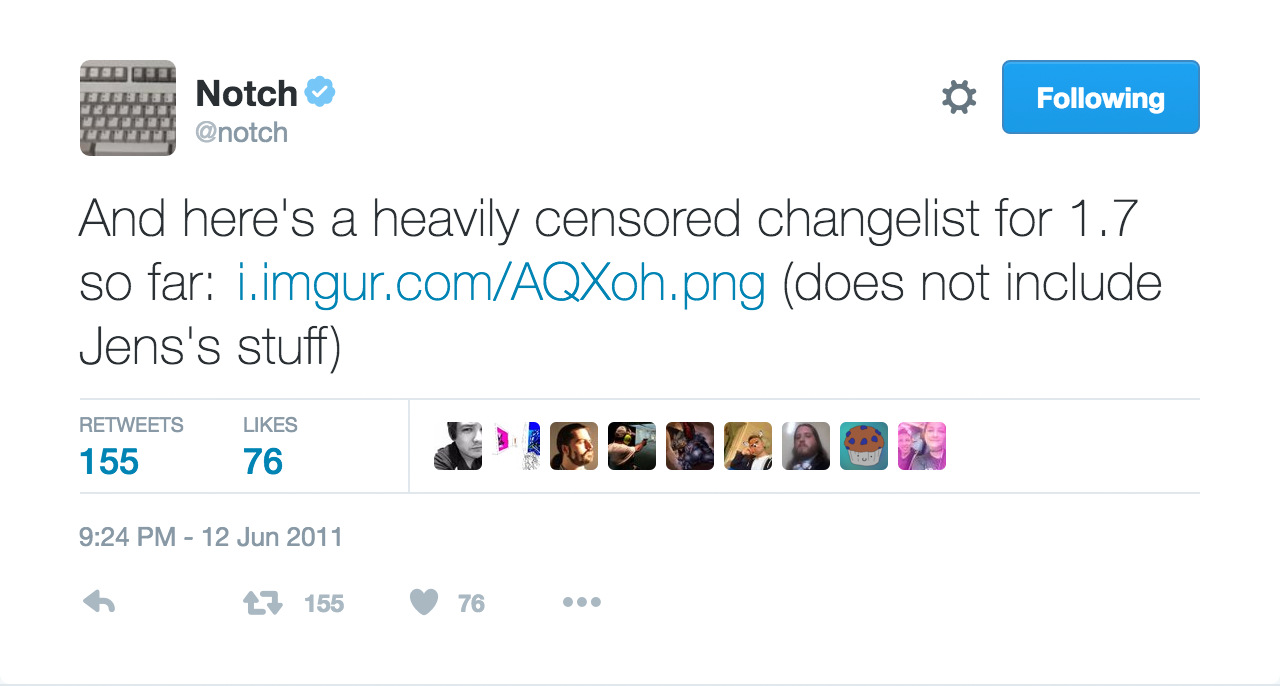
\includegraphics[width=0.7\textwidth]{fig/chapter1/notch_tweet.png}
    \caption[Print screen of Tweet from notch]{Print screen of Tweet from notch\protect\footnotemark}
    \label{ref:notch_twitter}
\end{figure}
\footnotetext{Tweet and image used with the consent of Markus Persson}

The image he is linking to can be seen in Figure \ref{fig:notch_imgur}. It is a print screen of what looks like a text editor or \gls{IDE}. The image is blurred, but only in a rectangular area in the middle of the image. Some of the text is still partially visible, like the lower portion of the file names in the tab pane at the top of the image. 

\begin{figure}[ht]
    \centering
    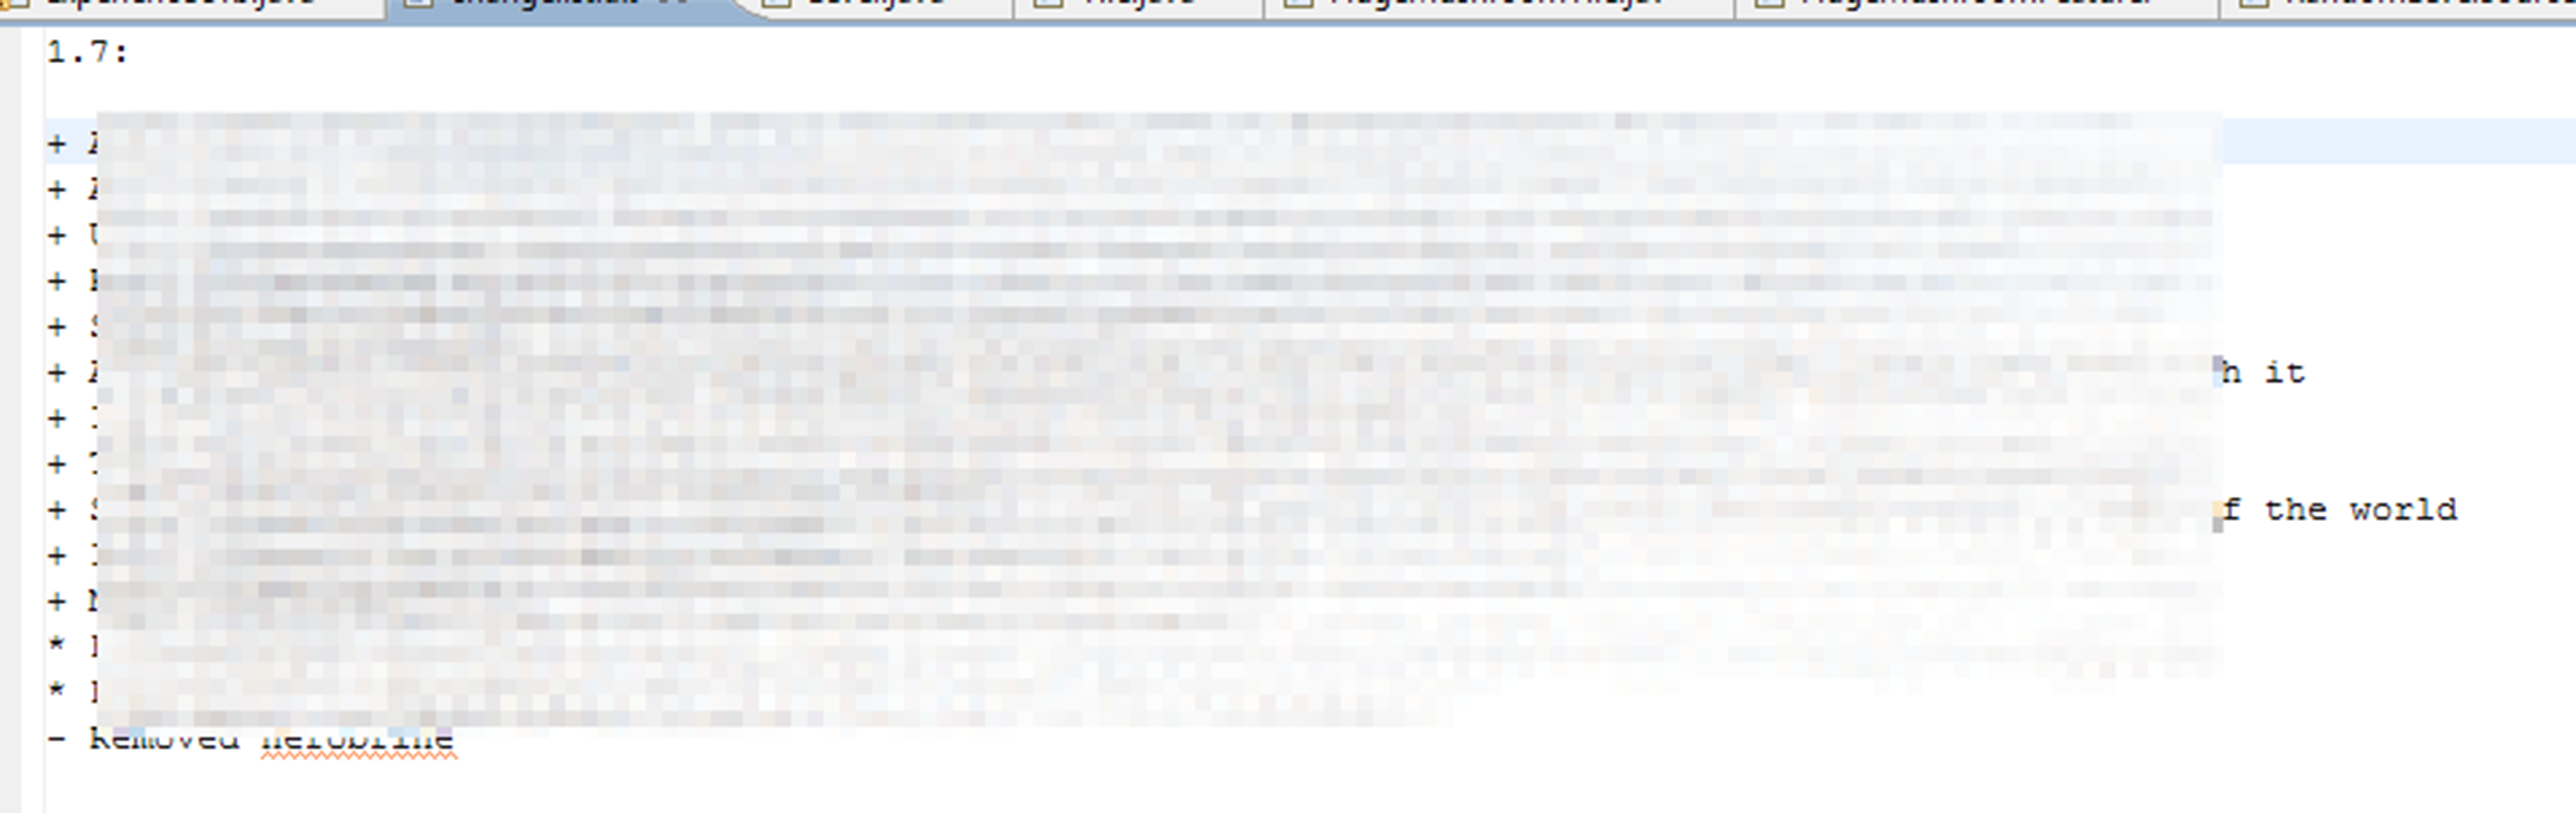
\includegraphics[width=0.7\textwidth]{fig/chapter1/notch_eclipse.png}
    \caption{Blurred image of Minecraft 1.7 changelog from @notch's Tweet}
    \label{fig:notch_imgur}
\end{figure}

The most interesting part about this image is the text in the tab pane, where only the lower portion of the characters are visible. When this image circulated the Internet, one user was able to identify the text in the tabs. He installed the \gls{IDE} Persson used, and compared the default font in the program to the image. His findings can be seen in in Figure \ref{fig:notch_eclipse_decoded}. More than four months later, when version 1.7 was released, it was confirmed that the decoding was correct, with the introduction of big mushrooms in the game\footnote{Experience Orbs were postponed, and introduced in the 1.8 update instead.} \cite{misc-minecraft.172-changelog}.

\begin{figure}[ht]
    \centering
    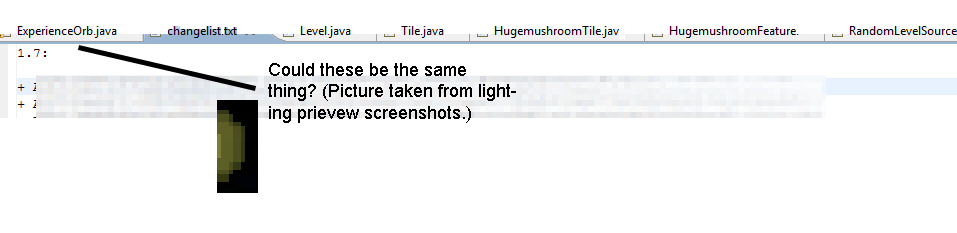
\includegraphics[width=0.7\textwidth]{fig/chapter1/notch_eclipse_decoded.png}
    \caption{Decoding the blurred image from Notch}
    \label{fig:notch_eclipse_decoded}
\end{figure}

Recalling seeing this posted online got the author thinking ``how could one use OCR and artificial intelligence to identify this text"? Would it even be possible? Because so little of the characters were present, regular OCR approaches would most likely not be able to give a correct classification. These questions lead to this thesis.